\begin{problem}{통신망 분할}
    {표준 입력}{표준 출력}
    {1 초}{512 MB}{}
    
    BOJ의 인기스타, 방송인 권욱제는 통신 회사에 취업했다. 현재 이 통신 회사는 너무나 큰 통신망을 한 지사에서 관리하느라 큰 비용을 지불하고 있었다. 그래서 회사는 최근 IT의 트렌드 중 하나인 `탈중앙화'에 편승하여, 통신망을 분할하도록 결정했다. 그래서 욱제한테 통신망을 분할 할때 발생하는 비용을 분석하도록 지시했다.

    현재 회사 망에는 1번부터 $ N $번까지 총 $ N $개의 통신 탑이 존재하며, 통신탑 간의 연결이 $ M $개 존재한다. 이때 회사에서는 총 $ Q $번 통신탑 간의 연결을 제거함으로써 하나의 통신망을 여러 개의 통신망으로 분리하려고 한다. 통신망이란, 통신탑의 연결을 통해 도달 가능한 통신탑들의 집합이다. 통신탑 간의 연결 관계를 제거할 때 드는 비용은 제거한 후 통신망이 두 개로 나누어진다면 나눠진 두 개의 통신망에 속한 통신탑들의 갯수의 곱이 되며, 나누어지지 않을 경우 0이다.
    
    \begin{figure}[h]
        \centering
        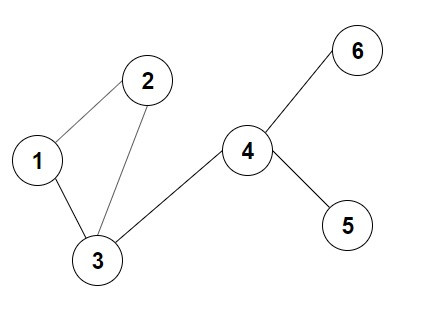
\includegraphics[width=0.4\textwidth]{network.jpg}
        \caption{예시 그래프}
    \end{figure}

    위의 그림을 예시로 할때, $ (3, 4)$ 간의 연결을 제거하면 $ \{1,\ 2,\ 3\} $, $ \{4,\ 5,\ 6\} $으로 분할 되며, 이때 발생하는 비용은 $ 3 \times 3 = 9 $가 된다. 대신 $ (2, 3) $ 간의 연결을 제거하면, 망이 나눠지지 않았기에 비용은 0이 된다.

    욱제는 회사의 요청에 따라 $ Q $번의 제거를 통해 나오는 비용의 합을 구해야 한다. 하지만 욱제는 회사의 통신망을 이용해 방송하기 바쁘기 때문에 우리가 도와주자.
    
    \InputFile
    
    첫 번째 줄에는 통신탑의 개수인 자연수 $ N $, 통신탑 사이의 연결의 개수인 자연수 $ M $, 통신망 연결 분할 횟수인 자연수 $ Q $가 공백으로 구분되어 주어진다. ($ 1 \leq N \leq 100,000 $, $ 1 \leq M \leq 100,000 $, $ 1 \leq Q \leq M $)
    
    두 번째 줄부터 $ M $개의 줄에 걸쳐 두 개의 자연수 $ X $, $ Y $가 공백으로 구분되어 주어진다. 이는 $ X $ 통신탑과 $ Y $ 통신탑 사이에 연결이 있음을 뜻한다. ($ 1 \leq X,\ Y \leq N $, $ X \neq Y $)
    
    중복된 연결은 주어지지 않으며, 모든 통신탑은 처음엔 하나의 통신망에 속한다. 조건에 의해 자기 자신과 연결이 있는 통신탑은 없다.
    
    그 다음 줄부터 $ Q $개의 줄에 걸쳐 제거될 연결의 번호인 자연수 $ A $가 주어진다. 이는 $ A $번째로 입력된 $ (X,\ Y) $의 연결이 제거되었음을 의미한다. ($ 1 \leq A \leq M $)
    
    이미 제거된 연결은 다시 제거되지 않으며, 제거는 입력 순서대로 진행된다.
    
    
    \OutputFile
    첫 번째 줄에 $ Q $개의 연결을 순서대로 제거하는데 드는 비용의 합을 출력한다.
    
    \Examples
    
    \begin{example}
        \exmp{
            4 4 3
            1 2
            2 3
            3 4
            1 4
            4
            2
            3
        }{%
            5
        }%
    \end{example}
        
    \Explanation
    첫 번째로 제거되는 연결은 $ (1, 4) $로, 통신망 $ \{1,\ 2,\ 3,\ 4\} $가 분리되지 않아 비용이 0이다.
    
    두 번째로 제거되는 연결은 $ (2, 3) $으로, 통신망 $ \{1,\ 2,\ 3,\ 4\} $가 $ \{1,\ 2\} $와 $ \{3,\ 4\} $로 분리되어 비용이 $ 2 \times 2 = 4 $이다.
    
    세 번째로 제거되는 연결은 $ (3, 4) $로, 통신망 $ \{3,\ 4\} $가 $ \{3\} $과 $ \{4\} $로 분리되어 비용이 $ 1 \times 1 = 1 $이다.
    
    결과적으로 총 비용은 $ 0 + 4 + 1 = 5 $이다.
    
\end{problem}

